\documentclass[20pt]{extarticle}

\usepackage[utf8]{inputenc}
\usepackage{color}
\usepackage[x11names]{xcolor}
\usepackage{geometry}
\usepackage{amsmath}
\usepackage{amssymb}
\usepackage{amsthm}
\usepackage{graphicx}
\usepackage{wrapfig}
\usepackage{subfig}
\usepackage{bm}
\usepackage{multirow}
\usepackage{array}
\usepackage{csquotes}
\usepackage{cmbright}
\usepackage{tikz}
\usepackage{pgfplots}
\pgfplotsset{compat = 1.17}
\usetikzlibrary{3d, graphs, shapes.geometric,decorations, arrows, positioning, arrows.meta, calc}
\color{white}

\geometry{
    a3paper,
    left = 0.5cm,
    right = 5.5cm,
    top = 0.5cm,
    bottom = 0.5cm
}

\thispagestyle{empty}  
\begin{document}


% \begin{displaymath}
%     E \overset{\mathrm{iid}}{\sim} N(0, \sigma^2)
% \end{displaymath}

% \begin{tikzpicture}[
%     node distance=1.5cm, % Distance between nodes
%     every node/.style={draw, rectangle}, % Default node style
%     dashednode/.style={draw, rectangle, dashed} % Dashed rectangle style
% ]


% % Nodes
% \node (Z) [dashednode] {OKÄND};
% \node (X) [below left=of Z] {Filmer};
% \node (Y) [below right=of Z] {Drunkningsolyckor};

% % Edges
% \draw (Z) -- (Y) [-{Stealth[length=3mm, width=2mm]}];
% \draw (Z) -- (X) [-{Stealth[length=3mm, width=2mm]}];
% \draw [-{Stealth[length=3mm, width=2mm]}] (X) -- (Y);

% % Aligning Filmer and Dödsfall on the same level
% \coordinate (Midpoint) at ($(X)!0.5!(Y)$);
% \draw [draw=none] (Midpoint) -- ++(0,-0.01) coordinate (align1);
% \draw [draw=none] (Midpoint) -- ++(0,0.01) coordinate (align2);
% \path [draw=none] (align1) edge[draw=none] (align2);

% \end{tikzpicture}

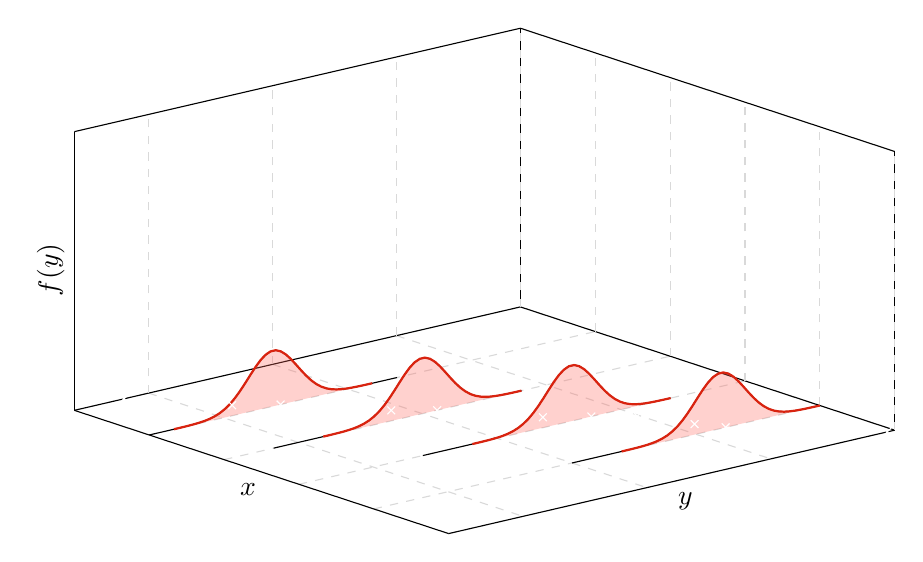
\begin{tikzpicture}
    % Scatter plot settings
    \begin{axis}[
        view={50}{30}, % Adjusted viewpoint slightly to the right
        domain=0:10, 
        samples=100,
        xlabel={$x$},
        ylabel={$y$},
        zlabel={$f(y)$},
        xtick align = outside,
        xmajorticks = false,
        ymajorticks = false,
        ytick align = outside,
        zmajorgrids = false,
        ztick = \empty,
        axis on top = false,
        grid=major,
        grid style = {dashed, gray!30},
        width=12cm, 
        height=8cm,
        scatter/classes={
            a={mark=x,draw=white,fill=white}
        },
        colormap/viridis,
        zmin = 0,
        zmax = 5
    ]

    % Scatter points (random observations along the line y = 4 + 1.5x)
    \addplot3[only marks, scatter, scatter src=explicit symbolic] 
        coordinates {
            (0, 4, 0)   [a]
            (1, 5.2, 0) [a]
            (2, 7.3, 0) [a]
            (3, 8.7, 0) [a]
            (4, 10.6, 0) [a]
            (5, 11.5, 0) [a]
            (6, 13.8, 0) [a]
            (7, 14.4, 0) [a]
            (8, 16.2, 0) [a]
            (9, 17.9, 0) [a]
            (10, 19.7, 0) [a]
            (1.5, 6.1, 0) [a]
            (2.5, 7.6, 0) [a]
            (3.5, 9.5, 0) [a]
            (4.5, 11.3, 0) [a]
            (5.5, 12.6, 0) [a]
            (6.5, 14.9, 0) [a]
            (7.5, 15.7, 0) [a]
            (8.5, 17.3, 0) [a]
            (9.5, 18.6, 0) [a]
        };

    % Normal distribution at x = 2
    \addplot3[fill= {rgb,255:red,255;green,102;blue,92}, fill opacity = 0.3, domain=2:12,samples=40] 
        ({2}, {y}, {exp(-0.5*((y-7)^2))});
    \addplot3[thick, color={rgb,255:red,217;green,35;blue,15}, domain=7-4:7+4, samples=40] 
        ({2}, {y}, {exp(-0.5*((y-7)^2))});

    % Normal distribution at x = 4
    \addplot3[fill= {rgb,255:red,255;green,102;blue,92}, fill opacity = 0.3, domain=4:14,samples=40] 
        ({4}, {y}, {exp(-0.5*((y-10)^2))});
    \addplot3[thick, color={rgb,255:red,217;green,35;blue,15}, domain=10-4:10+4, samples=40] 
        ({4}, {y}, {exp(-0.5*((y-10)^2))});

    % Normal distribution at x = 6
    \addplot3[fill= {rgb,255:red,255;green,102;blue,92}, fill opacity = 0.3, domain=7:17,samples=40] 
        ({6}, {y}, {exp(-0.5*((y-13)^2))});
    \addplot3[thick, color={rgb,255:red,217;green,35;blue,15}, domain=13-4:13+4, samples=40] 
        ({6}, {y}, {exp(-0.5*((y-13)^2))});
    
        % Normal distribution at x = 8
    \addplot3[fill= {rgb,255:red,255;green,102;blue,92}, fill opacity = 0.3, domain=10:20,samples=40] 
        ({8}, {y}, {exp(-0.5*((y-16)^2))});
    \addplot3[thick, color={rgb,255:red,217;green,35;blue,15}, domain=16-4:16+4, samples=40] 
        ({8}, {y}, {exp(-0.5*((y-16)^2))});
    


    \end{axis}
    
    \end{tikzpicture}

\end{document}